\subsection{Polarización}

\par Se realizaron las mediciones de punto de polarización del amplificador sin señal aplicada, obteniéndose los resultados de la tabla ~\tableref{tab:PuntoQ1}. Los mismos se verificaron con y sin la carga conectada para observar que no haya cambios en la polarización, una vez ajustada la corriente de polarización de salida.


%\begin{table}[H]
%    \setlength\arrayrulewidth{1pt}
%    \arrayrulecolor{TABLEColor}
%    \begin{center}
%        \begin{tabular}{llllll}
%        \hline\hline
%            Transistor & $V_{CEQ}$ & $I_{CQ}$ & $P_{max}$\\
%            \hline \hline
%            Q1 (BC546C)     &33.V	&529uV	&17.7mV    \\
%            Q2 (BC556B)     &1.27V	&528uV	&671uV    \\
%            Q3 (BC546B)     &31.6V	&1.07mV	&33.8mV    \\
%            Q4 (BC556B)     &612mV	&5.32mV	&326uV    \\
%            Q5 (BC546B)     &34.3V	&5.38uV	&18.4mV    \\
%            Q6 (BC546B)     &28.9V	&9.73mV	&282mV    \\
%            Q7 (BC556B)     &28.3V	&146uV	&4.12mV    \\
%            Q8 (BC556B)     &29.9V	&9.60mV	&287mV    \\
%            Q9 (BD135)      &2.95V	&9.40mV	&27.7mV    \\
%            Q10(BD136)      &14.2V	&0	        &0    \\
%            Q11(BD136)      &19.8V	&0	        &0    \\
%            Q12(BD135)      &20.0V	&0	        &0   \\
%            Q13(BD135)      &14.4V	&0	        &0   \\
%            Q14(MJL21194)   &20.0V	&0	        &0   \\
%            Q15(MJL21194)   &1.50V	&0	        &0    \\
%            Q16(MJL21193)   &14.9V	&0	        &0   \\
%            Q17(MJL21193)   &20.2V	&0	        &0    \\
%            Q18(2N3906)     &1.27V	&0	        &0   \\
%            Q19(2N3904)     &1.26V	&0	        &0    \\
%        \end{tabular}
%    \caption{Q2}
%    \label{tab:PuntoQ}
%    \end{center}
%\end{table}
%
%
%
%\begin{table}[H]
%    \setlength\arrayrulewidth{1pt}
%    \arrayrulecolor{TABLEColor}
%    \begin{center}
%        \begin{tabular}{llllll}
%        \hline\hline
%            Transistor & $V_{CEQ}$ & $I_{CQ}$ & $P_{max}$\\
%            \hline \hline
%            Q1 (BC546C)     & 33.9V     & 549uA     & 18.6mW    \\
%            Q2 (BC556B)     & 1.31V     & 549uA     & 721uW     \\
%            Q3 (BC546B)     & 31.8V     & 1.1mA     & 35mW      \\
%            Q4 (BC556B)     & 61.1V     & 549uA     & 334mW     \\
%            Q5 (BC546B)     & 34.6V     & 549uA     & 19mW      \\
%            Q6 (BC546B)     & 28.9V     & 9.71mA    & 281mW     \\
%            Q7 (BC556B)     & 30.2V     & 169uA     & 5.12mW       \\
%            Q8 (BC556B)     & 30.9V     & 9.55mA    & 295mW     \\ 
%            Q9 (BD135)      & 2.63V     & 9.48mA    & 28mW      \\
%            Q10(BD136)      & 14.1V     & 7.02mA    & 208mW     \\
%            Q11(BD136)      & 20.2V     & 0         & 0     \\
%            Q12(BD135)      & 20.2V     & 0         & 0     \\
%            Q13(BD135)      & 14.1V     & 7.84mA    & 111mW     \\
%            Q14(MJL21194)   & 20.2V     & 0         & 0     \\
%            Q15(MJL21194)   & 14.8V     & 92.3mA    & 1.36W    \\
%            Q16(MJL21193)   & 14.8V     & 93.2mA    & 1.38W    \\
%            Q17(MJL21193)   & 20.2V     & 0         & 0     \\
%            Q18(2N3906)     & 1.32V     & 0         & 0     \\
%            Q19(2N3904)     & 1.31V     & 0         & 0     \\\hline\hline
%        \end{tabular}
%    \caption{Q1}
%    \label{tab:PuntoQ}
%    \end{center}
%\end{table}





\begin{table}[H]  %%\centering
    
    \setlength\arrayrulewidth{1.5pt}
    \arrayrulecolor{white}
    \def\clinecolor{\hhline{|>{\arrayrulecolor{white}}-%
    >{\arrayrulecolor{white}}|-|-|-|-|-|}}
    
\begin{center}  
\resizebox{0.7 \textwidth}{!}{%    
\begin{tabularx}{1 \textwidth}%
    {|
    >{\columncolor{white} \centering\arraybackslash}m{0.3333\linewidth}
     |
    >{\columncolor{white} \centering\arraybackslash}m{0.1667\linewidth}
     |
    >{\columncolor{white} \centering\arraybackslash}m{0.1667\linewidth}
     |
    >{\columncolor{white} \centering\arraybackslash}m{0.1667\linewidth}
     |
    >{\columncolor{white} \centering\arraybackslash}m{0.1667\linewidth}
     |
    }
    \rowcolor{HeadersColor} \thead{Transistor} & \thead{$V_{CE_{Q}}$} & \thead{$I_{C_{Q}}$} & \thead{ $P_{Q}$}\\    
    \hhline{|-|-|-|-|-|}
    %\rowcolor{Butter!20} \cellcolor{Butter!40} $I_{C}$ [$\si[per-mode=symbol]{\milli\ampere}$] & $0.54$ & $8.66$ & $9$ & $6$ & $5.5$ & $10$ & $10$  \\
    % \hhline{|-|-|-|-|-|}
    \rowcolor{gray!20} \cellcolor{gray!40} $Q_{1}$ (BC546C) & $0 \si[per-mode=symbol]{\volt}$  & $0 \si[per-mode=symbol]{\milli\ampere}$ & $ 0\si[per-mode=symbol]{\milli\watt}$ \\
    \hhline{|-|-|-|-|-|}
    \rowcolor{gray!20} \cellcolor{gray!40} $Q_{2}$ (BC556B) & $0 \si[per-mode=symbol]{\volt}$  & $0 \si[per-mode=symbol]{\milli\ampere}$ & $ 0\si[per-mode=symbol]{\milli\watt}$ \\
    \hhline{|-|-|-|-|-|}
    \rowcolor{gray!20} \cellcolor{gray!40} $Q_{3}$ (BC546B) & $0 \si[per-mode=symbol]{\volt}$  & $0 \si[per-mode=symbol]{\milli\ampere}$ & $ 0\si[per-mode=symbol]{\milli\watt}$ \\
    \hhline{|-|-|-|-|-|}
    \rowcolor{gray!20} \cellcolor{gray!40} $Q_{4}$ (BC556B) & $0 \si[per-mode=symbol]{\volt}$  & $0 \si[per-mode=symbol]{\milli\ampere}$ & $ 0\si[per-mode=symbol]{\milli\watt}$ \\
    \hhline{|-|-|-|-|-|}
    \rowcolor{gray!20} \cellcolor{gray!40} $Q_{5}$ (BC546B) & $0 \si[per-mode=symbol]{\volt}$  & $0 \si[per-mode=symbol]{\milli\ampere}$ & $ 0\si[per-mode=symbol]{\milli\watt}$ \\
    \hhline{|-|-|-|-|-|}
    \rowcolor{gray!20} \cellcolor{gray!40} $Q_{6}$ (BC546B) & $0 \si[per-mode=symbol]{\volt}$  & $0 \si[per-mode=symbol]{\milli\ampere}$ & $ 0\si[per-mode=symbol]{\milli\watt}$ \\
    \hhline{|-|-|-|-|-|}
    \rowcolor{gray!20} \cellcolor{gray!40} $Q_{7}$ (BC556B) & $0 \si[per-mode=symbol]{\volt}$  & $0 \si[per-mode=symbol]{\milli\ampere}$ & $ 0\si[per-mode=symbol]{\milli\watt}$ \\
    \hhline{|-|-|-|-|-|}
    \rowcolor{gray!20} \cellcolor{gray!40} $Q_{8}$ (BC556B) & $0 \si[per-mode=symbol]{\volt}$  & $0 \si[per-mode=symbol]{\milli\ampere}$ & $ 0\si[per-mode=symbol]{\milli\watt}$ \\
    \hhline{|-|-|-|-|-|}
    \rowcolor{gray!20} \cellcolor{gray!40} $Q_{9}$ (BD135) & $0 \si[per-mode=symbol]{\volt}$  & $0 \si[per-mode=symbol]{\milli\ampere}$ & $ 0\si[per-mode=symbol]{\milli\watt}$ \\
    \hhline{|-|-|-|-|-|}
    \rowcolor{gray!20} \cellcolor{gray!40} $Q_{10}$(BD136) & $0 \si[per-mode=symbol]{\volt}$  & $0 \si[per-mode=symbol]{\milli\ampere}$ & $ 0\si[per-mode=symbol]{\milli\watt}$ \\
    \hhline{|-|-|-|-|-|}
    \rowcolor{gray!20} \cellcolor{gray!40} $Q_{11}$(BD136) & $0 \si[per-mode=symbol]{\volt}$  & $0 \si[per-mode=symbol]{\milli\ampere}$ & $ 0\si[per-mode=symbol]{\milli\watt}$ \\
    \hhline{|-|-|-|-|-|}
    \rowcolor{gray!20} \cellcolor{gray!40} $Q_{12}$(BD135) & $0 \si[per-mode=symbol]{\volt}$  & $0 \si[per-mode=symbol]{\milli\ampere}$ & $ 0\si[per-mode=symbol]{\milli\watt}$ \\
    \hhline{|-|-|-|-|-|}
    \rowcolor{gray!20} \cellcolor{gray!40} $Q_{13}$(BD135) & $0 \si[per-mode=symbol]{\volt}$  & $0 \si[per-mode=symbol]{\milli\ampere}$ & $ 0\si[per-mode=symbol]{\milli\watt}$ \\
    \hhline{|-|-|-|-|-|}
    \rowcolor{gray!20} \cellcolor{gray!40} $Q_{14}$(MJL21194) & $0 \si[per-mode=symbol]{\volt}$  & $0 \si[per-mode=symbol]{\milli\ampere}$ & $ 0\si[per-mode=symbol]{\milli\watt}$ \\
    \hhline{|-|-|-|-|-|}
    \rowcolor{gray!20} \cellcolor{gray!40} $Q_{15}$(MJL21194) & $0 \si[per-mode=symbol]{\volt}$  & $0 \si[per-mode=symbol]{\milli\ampere}$ & $ 0\si[per-mode=symbol]{\milli\watt}$ \\
    \hhline{|-|-|-|-|-|}
    \rowcolor{gray!20} \cellcolor{gray!40} $Q_{16}$(MJL21193) & $0 \si[per-mode=symbol]{\volt}$  & $0 \si[per-mode=symbol]{\milli\ampere}$ & $ 0\si[per-mode=symbol]{\milli\watt}$ \\
    \hhline{|-|-|-|-|-|}
    \rowcolor{gray!20} \cellcolor{gray!40} $Q_{17}$(MJL21193) & $0 \si[per-mode=symbol]{\volt}$  & $0 \si[per-mode=symbol]{\milli\ampere}$ & $ 0\si[per-mode=symbol]{\milli\watt}$ \\
    \hhline{|-|-|-|-|-|}
    \rowcolor{gray!20} \cellcolor{gray!40} $Q_{18}$(2N3906) & $0 \si[per-mode=symbol]{\volt}$  & $0 \si[per-mode=symbol]{\milli\ampere}$ & $ 0\si[per-mode=symbol]{\milli\watt}$ \\
    \hhline{|-|-|-|-|-|}
    \rowcolor{gray!20} \cellcolor{gray!40} $Q_{19}$(2N3904) &$0 \si[per-mode=symbol]{\volt}$  & $0 \si[per-mode=symbol]{\milli\ampere}$ & $ 0\si[per-mode=symbol]{\milli\watt}$ \\
    \hhline{|-|-|-|-|-|}            
    \end{tabularx}}
	\caption{Primer punto de operación.}
    \label{tab:PuntoQ1}
	\end{center}
\end{table}


\begin{table}[H]  %%\centering
    
    \setlength\arrayrulewidth{1.5pt}
    \arrayrulecolor{white}
    \def\clinecolor{\hhline{|>{\arrayrulecolor{white}}-%
    >{\arrayrulecolor{white}}|-|-|-|-|-|}}
    
\begin{center}  
\resizebox{0.7 \textwidth}{!}{%    
\begin{tabularx}{1 \textwidth}%
    {|
    >{\columncolor{white} \centering\arraybackslash}m{0.3333\linewidth}
     |
    >{\columncolor{white} \centering\arraybackslash}m{0.1667\linewidth}
     |
    >{\columncolor{white} \centering\arraybackslash}m{0.1667\linewidth}
     |
    >{\columncolor{white} \centering\arraybackslash}m{0.1667\linewidth}
     |
    >{\columncolor{white} \centering\arraybackslash}m{0.1667\linewidth}
     |
    }
    \rowcolor{HeadersColor} \thead{Transistor} & \thead{$V_{CE_{Q}}$} & \thead{$I_{C_{Q}}$} & \thead{ $P_{Q}$}\\    
    \hhline{|-|-|-|-|-|}
    %\rowcolor{Butter!20} \cellcolor{Butter!40} $I_{C}$ [$\si[per-mode=symbol]{\milli\ampere}$] & $0.54$ & $8.66$ & $9$ & $6$ & $5.5$ & $10$ & $10$  \\
    % \hhline{|-|-|-|-|-|}
    \rowcolor{gray!20} \cellcolor{gray!40} $Q_{1}$ (BC546C) & $0 \si[per-mode=symbol]{\volt}$  & $0 \si[per-mode=symbol]{\milli\ampere}$ & $ 0\si[per-mode=symbol]{\milli\watt}$ \\
    \hhline{|-|-|-|-|-|}
    \rowcolor{gray!20} \cellcolor{gray!40} $Q_{2}$ (BC556B) & $0 \si[per-mode=symbol]{\volt}$  & $0 \si[per-mode=symbol]{\milli\ampere}$ & $ 0\si[per-mode=symbol]{\milli\watt}$ \\
    \hhline{|-|-|-|-|-|}
    \rowcolor{gray!20} \cellcolor{gray!40} $Q_{3}$ (BC546B) & $0 \si[per-mode=symbol]{\volt}$  & $0 \si[per-mode=symbol]{\milli\ampere}$ & $ 0\si[per-mode=symbol]{\milli\watt}$ \\
    \hhline{|-|-|-|-|-|}
    \rowcolor{gray!20} \cellcolor{gray!40} $Q_{4}$ (BC556B) & $0 \si[per-mode=symbol]{\volt}$  & $0 \si[per-mode=symbol]{\milli\ampere}$ & $ 0\si[per-mode=symbol]{\milli\watt}$ \\
    \hhline{|-|-|-|-|-|}
    \rowcolor{gray!20} \cellcolor{gray!40} $Q_{5}$ (BC546B) & $0 \si[per-mode=symbol]{\volt}$  & $0 \si[per-mode=symbol]{\milli\ampere}$ & $ 0\si[per-mode=symbol]{\milli\watt}$ \\
    \hhline{|-|-|-|-|-|}
    \rowcolor{gray!20} \cellcolor{gray!40} $Q_{6}$ (BC546B) & $0 \si[per-mode=symbol]{\volt}$  & $0 \si[per-mode=symbol]{\milli\ampere}$ & $ 0\si[per-mode=symbol]{\milli\watt}$ \\
    \hhline{|-|-|-|-|-|}
    \rowcolor{gray!20} \cellcolor{gray!40} $Q_{7}$ (BC556B) & $0 \si[per-mode=symbol]{\volt}$  & $0 \si[per-mode=symbol]{\milli\ampere}$ & $ 0\si[per-mode=symbol]{\milli\watt}$ \\
    \hhline{|-|-|-|-|-|}
    \rowcolor{gray!20} \cellcolor{gray!40} $Q_{8}$ (BC556B) & $0 \si[per-mode=symbol]{\volt}$  & $0 \si[per-mode=symbol]{\milli\ampere}$ & $ 0\si[per-mode=symbol]{\milli\watt}$ \\
    \hhline{|-|-|-|-|-|}
    \rowcolor{gray!20} \cellcolor{gray!40} $Q_{9}$ (BD135) & $0 \si[per-mode=symbol]{\volt}$  & $0 \si[per-mode=symbol]{\milli\ampere}$ & $ 0\si[per-mode=symbol]{\milli\watt}$ \\
    \hhline{|-|-|-|-|-|}
    \rowcolor{gray!20} \cellcolor{gray!40} $Q_{10}$(BD136) & $0 \si[per-mode=symbol]{\volt}$  & $0 \si[per-mode=symbol]{\milli\ampere}$ & $ 0\si[per-mode=symbol]{\milli\watt}$ \\
    \hhline{|-|-|-|-|-|}
    \rowcolor{gray!20} \cellcolor{gray!40} $Q_{11}$(BD136) & $0 \si[per-mode=symbol]{\volt}$  & $0 \si[per-mode=symbol]{\milli\ampere}$ & $ 0\si[per-mode=symbol]{\milli\watt}$ \\
    \hhline{|-|-|-|-|-|}
    \rowcolor{gray!20} \cellcolor{gray!40} $Q_{12}$(BD135) & $0 \si[per-mode=symbol]{\volt}$  & $0 \si[per-mode=symbol]{\milli\ampere}$ & $ 0\si[per-mode=symbol]{\milli\watt}$ \\
    \hhline{|-|-|-|-|-|}
    \rowcolor{gray!20} \cellcolor{gray!40} $Q_{13}$(BD135) & $0 \si[per-mode=symbol]{\volt}$  & $0 \si[per-mode=symbol]{\milli\ampere}$ & $ 0\si[per-mode=symbol]{\milli\watt}$ \\
    \hhline{|-|-|-|-|-|}
    \rowcolor{gray!20} \cellcolor{gray!40} $Q_{14}$(MJL21194) & $0 \si[per-mode=symbol]{\volt}$  & $0 \si[per-mode=symbol]{\milli\ampere}$ & $ 0\si[per-mode=symbol]{\milli\watt}$ \\
    \hhline{|-|-|-|-|-|}
    \rowcolor{gray!20} \cellcolor{gray!40} $Q_{15}$(MJL21194) & $0 \si[per-mode=symbol]{\volt}$  & $0 \si[per-mode=symbol]{\milli\ampere}$ & $ 0\si[per-mode=symbol]{\milli\watt}$ \\
    \hhline{|-|-|-|-|-|}
    \rowcolor{gray!20} \cellcolor{gray!40} $Q_{16}$(MJL21193) & $0 \si[per-mode=symbol]{\volt}$  & $0 \si[per-mode=symbol]{\milli\ampere}$ & $ 0\si[per-mode=symbol]{\milli\watt}$ \\
    \hhline{|-|-|-|-|-|}
    \rowcolor{gray!20} \cellcolor{gray!40} $Q_{17}$(MJL21193) & $0 \si[per-mode=symbol]{\volt}$  & $0 \si[per-mode=symbol]{\milli\ampere}$ & $ 0\si[per-mode=symbol]{\milli\watt}$ \\
    \hhline{|-|-|-|-|-|}
    \rowcolor{gray!20} \cellcolor{gray!40} $Q_{18}$(2N3906) & $0 \si[per-mode=symbol]{\volt}$  & $0 \si[per-mode=symbol]{\milli\ampere}$ & $ 0\si[per-mode=symbol]{\milli\watt}$ \\
    \hhline{|-|-|-|-|-|}
    \rowcolor{gray!20} \cellcolor{gray!40} $Q_{19}$(2N3904) &$0 \si[per-mode=symbol]{\volt}$  & $0 \si[per-mode=symbol]{\milli\ampere}$ & $ 0\si[per-mode=symbol]{\milli\watt}$ \\
    \hhline{|-|-|-|-|-|}            
    \end{tabularx}}
	\caption{Segundo punto de operación.}
    \label{tab:PuntoQ2}
	\end{center}
\end{table}






\vfill

\clearpage


\subsection{Ancho de banda}

%\begin{figure}[H]
%    \centering
%    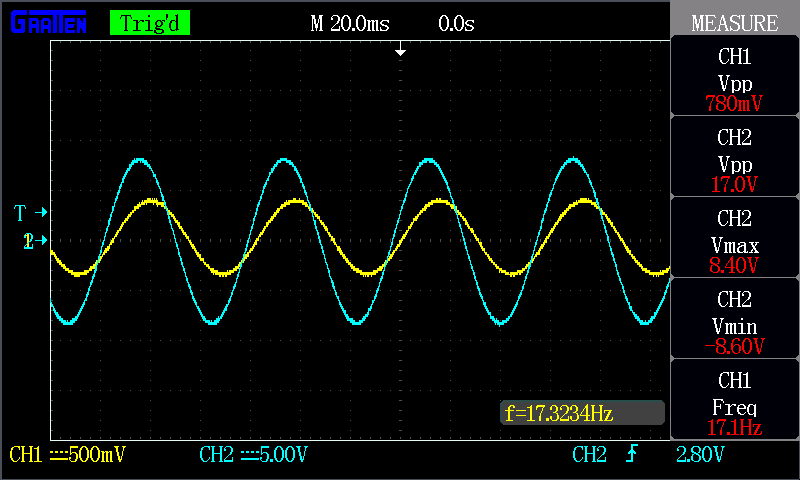
\includegraphics[angle=90,scale=0.8]{./img/mediciones/BW_low_power/1.png}
%    \caption{Ancho de banda a baja potencia}
%    \label{fig:PuntoQ_simulacion}
%\end{figure}

\subsection{Ancho de banda de potencia}

\subsection{Potencia}

\subsection{Sensibilidad}

\subsection{Slew Rate}

\subsection{THD}